\documentclass[tikz]{standalone}
\usepackage{pgfplots}
\pgfplotsset{compat=1.15}
\usepackage{mathrsfs}
\usetikzlibrary{arrows,calc}
\usepackage{tkz-euclide}
\pagestyle{empty}

\definecolor{AngleClr}{rgb}{0,0.39215686274509803,0}
\definecolor{ShapeClr}{rgb}{0.6,0.2,0}

\begin{document}

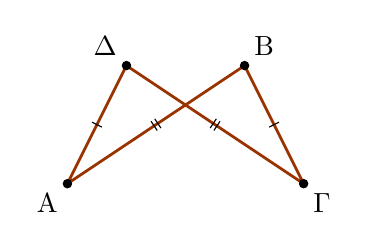
\begin{tikzpicture}[scale=.75]
\tkzSetUpLine[line width=1pt,color=black]
\tkzSetUpPoint[fill=black]

\tkzDefPoints{0/0/A,4/0/B,1/2/D,3/2/C}

\tkzFillPolygon[fill=white](A,C,B,D)

\tkzDrawPolygon[color=ShapeClr](A,C,B,D)
\tkzDrawPoints[size=3](A,B,C,D)
\tkzLabelPoint[below left](A){$\rm A$}
\tkzLabelPoint[below right](B){$\rm \Gamma$}
\tkzLabelPoint[above right](C){$\rm B$}
\tkzLabelPoint[above left](D){$\rm \Delta$}

\tkzMarkSegments[mark=|,size=2](A,D B,C)
\tkzMarkSegments[mark=||,size=2](A,C B,D)

\end{tikzpicture}
\end{document}
